\documentclass[11pt]{article}
\usepackage{setspace}  % To use linespacing
\usepackage{indentfirst} % Indents first line after sections
\usepackage{amssymb} % For \mathbb
\usepackage{enumerate} % For changing labels of enumerate
\usepackage[margin=1in]{geometry} % For editing margins
\usepackage{tikz} % Tikz drawing for graphs
\usetikzlibrary{arrows.meta} % Allows customizing arrows

\usepackage{amsmath}

% Make new commands
\newcommand{\N}{\mathbb{N}}
\newcommand{\R}{\mathbb{R}}
\newcommand{\Z}{\mathbb{Z}}
\newcommand{\abs}[1]{\left|#1\right|}
\newcommand{\fivespace}{\space\space\space\space\space}

% Start main document
\begin{document}
\onehalfspacing
\hfill Frank Cline

\hfill Math 307

\hfill HW 4

% Sections
% 3.4 # 1, 2, 5, 8, 17
% 3.5 # 2, 4, 5, 8, 12
% 11.1 # 1, 15acd, and look at hw4 pdf for another problem
% 11.2 # look online

% SECTION 3.4 # 1, 2, 5, 8, 17
\section*{3.4}
\begin{enumerate}
\item Which of the following describe equivalence relations? For those that are not equivalence relations, specify which of $(R),(S),(T)$ fail and illustrate the failures with examples.
	\begin{enumerate}
	\item $L_1||L_2$ for straight lines in the plane if $L_1$ and $L_2$ are the same or are parallel.\\
	Yes.
	\item $L_1\perp L_2$ for straight lines in the plane if $L_1$ and $L_2$ are perpendicular.\\
	No.\\
	Not $(R)$ because a straight line can never be perpendicular to itself. $L_1\not\perp L_1$.\\
	Not $(T)$ because if $L_1\perp L_2$ and $L_2\perp L_3$, then $L_1\not\perp L_3$. $L_1||L_3$.
	\item $p_1\sim p_2$ for Americans if $p_1$ and $p_2$ live in the same state.\\
	No. There are some Americans that don't live in a state like in Washington D.C.
	\item $p_1\approx p_2$ for Americans if $p_1$ and $p_2$ live in the same state or in neighboring 
	states.\\
	No. There are some Americans that don't live in a state like in Washington D.C.
	\item $p_1\approx p_2$ for people if $p_1$ and $p_2$ have a parent in common.\\
	No.\\
	Not $(T)$ because if $p_1\approx p_2$ and $p_2\approx p_3$, it doesn't mean $p_1\approx p_3$ because they could have 
	different parents.
	\item $p_1\cong p_2$ for people if $p_1$ and $p_2$ have the same mother.\\
	Yes.
	\end{enumerate}
\item For each example of an equivalence relation in Exercise 1, describe the members of some equivalence class.
	\begin{enumerate}
	\item $L_1||L_2$ for straight lines in the plane if $L_1$ and $L_2$ are the same or are parallel.\\
	If we describe the lines as vectors, then $[<1,1>]=\{<2,2>,<3,3>,<4,4>,...\}$.
	\setcounter{enumii}{5}
	\item $p_1\cong p_2$ for people if $p_1$ and $p_2$ have the same mother.\\
	The equivalence class of Michelle Obama is $[$Michelle$]=\{$Sasha, Malia$\}$.
	\end{enumerate}
\setcounter{enumi}{4}
\item If $G$ and $H$ are both graphs with vertex set $\{1,2,...,n\}$, we say that $G$ is isomorphic to $H$, and write $G\cong H$, in case there is a way to label the vertices of $G$ so that it becomes $H$.
\[
	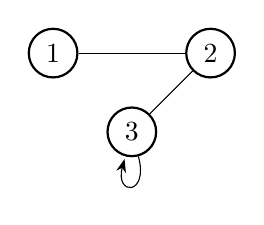
\begin{tikzpicture}
	\begin{scope}[every node/.style={circle,thick,draw}]
	    \node (1) at (0,0) {$1$};
	    \node (2) at (2,0) {$2$};
	    \node (3) at (1,-1) {$3$};
	\end{scope}
	
	\begin{scope}[>={Stealth[black]},
	              every node/.style={fill=white,circle},
	              every edge/.style={draw=black}]
	    	\path (1) edge (2);
	    	\path (2) edge (3);
		\path (3) edge[loop below] (3);
	\end{scope}
	\end{tikzpicture}
	\simeq
	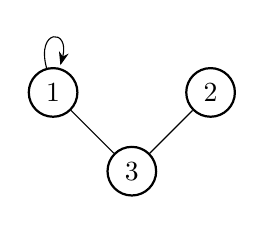
\begin{tikzpicture}
	\begin{scope}[every node/.style={circle,thick,draw}]
	    \node (1) at (0,0) {$1$};
	    \node (2) at (2,0) {$2$};
	    \node (3) at (1,-1) {$3$};
	\end{scope}
	
	\begin{scope}[>={Stealth[black]},
	              every node/.style={fill=white,circle},
	              every edge/.style={draw=black}]
	    	\path (1) edge[loop above] (1);
	    	\path (1) edge (3);
		\path (3) edge (2);
	\end{scope}
	\end{tikzpicture}
\]
	\begin{enumerate}
	\item Give a picture of another graph isomorphic to these two.\\
		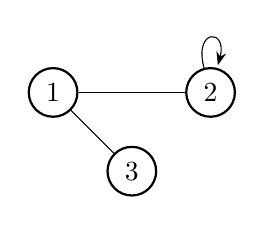
\begin{tikzpicture}
		\begin{scope}[every node/.style={circle,thick,draw}]
		    \node (1) at (0,0) {$1$};
		    \node (2) at (2,0) {$2$};
		    \node (3) at (1,-1) {$3$};
		\end{scope}
		
		\begin{scope}[>={Stealth[black]},
		              every node/.style={fill=white,circle},
		              every edge/.style={draw=black}]
		    	\path (1) edge (2);
		    	\path (1) edge (3);
			\path (2) edge[loop above] (2);
		\end{scope}
		\end{tikzpicture}
	\item Find a graph with vertex set $\{1,2,3\}$ that is not isomorphic to the graphs yet has three edges and exactly one is 
	a loop.\\
		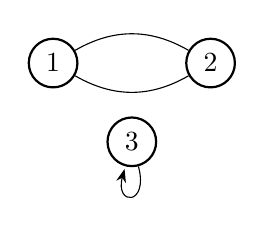
\begin{tikzpicture}
		\begin{scope}[every node/.style={circle,thick,draw}]
		    \node (1) at (0,0) {$1$};
		    \node (2) at (2,0) {$2$};
		    \node (3) at (1,-1) {$3$};
		\end{scope}
		
		\begin{scope}[>={Stealth[black]},
		              every node/.style={fill=white,circle},
		              every edge/.style={draw=black}]
		    	\path (1) edge[bend right=30] (2);
		    	\path (1) edge[bend left=30] (2);
			\path (3) edge[loop below] (3);
		\end{scope}
		\end{tikzpicture}
	\item Find another example as in part(b) that isn't isomorphic to the answer of part(b) and the other two graphs.\\
		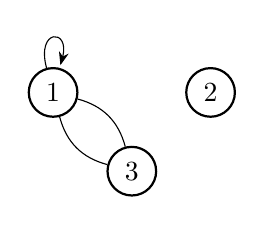
\begin{tikzpicture}
		\begin{scope}[every node/.style={circle,thick,draw}]
		    \node (1) at (0,0) {$1$};
		    \node (2) at (2,0) {$2$};
		    \node (3) at (1,-1) {$3$};
		\end{scope}
		
		\begin{scope}[>={Stealth[black]},
		              every node/.style={fill=white,circle},
		              every edge/.style={draw=black}]
		    	\path (1) edge[bend right=30] (3);
		    	\path (1) edge[bend left=30] (3);
			\path (1) edge[loop above] (1);
		\end{scope}
		\end{tikzpicture}
	\item Show that $\simeq$ is an equivalence relation on the set of all graphs with the vertex set $\{1,2,...,n\}$.\\
	DO WORK HERE.
	\end{enumerate}
\setcounter{enumi}{7}
\item
	\begin{enumerate}
	\item For $m,n\in\Z$, define $m\sim n$ in case $m-n$ is odd. Is the relation reflexive? symmetric? transitive? Is it an 
	equivalence relation?\\
	$(R)$ No because if $n=m$, then $m-n$ is 0, and zero is even, so $m\not\sim n$ thus the relation is not 
	reflexive.\\
	$(S)$ Yes because $\forall m,n\in\Z$ if $m-n=odd$, then $n-m=-odd$ thus the relation is symmetric.\\
	$(T)$ No. Suppose $m=6,n=3$ and $\exists a\in\Z:a=2$ then $m-n=3$ and $n-a=1$, so $m\sim n$ and $n\sim a$. However, 
	$m-a=4$ so $m\not\sim a$ thus the relation is not transitive.\\
	It is not an equivalence relation because the relation is not reflexive or transitive.
	\item For $a$ and $b$ in $\R$, define $a\sim b$ in case $|a-b|\leq 1$. One could say that $a\sim b$ in case $a$ and $b$ are 
	close enough or approximately equal. Answer the question in part (a).\\
	$(R)$ Yes because if $a=b$ then $a-b=0\leq1$ so $a\sim b$ thus the relation is reflexive.\\
	$(S)$ Yes because $|a-b|=|b-a|$ so if $a\sim b$ then $b\sim a$ thus the relation is symmetric\\
	$(T)$ No. Suppose $a=10,b=9$, and $\exists c\in\R:c=8$. $a-b=1$ and $b-c=1$ so $a\sim b$ and $b\sim c$. However, $a-c=2$ thus 	the relation is not transitive because $a\sim b\wedge b\sim c$ but $a\not\sim c$.\\
	It is not an equivalence relation because the relation is not transitive.
	\end{enumerate}
\setcounter{enumi}{16}
\item 
	\begin{enumerate}
	\item Verify that the relation $\cong$ defined in Example 5b (the reachable Relation $R$ on $V(G)$ by $(v,w)\in R$) is an 
	equivalence relation on $V(G)$.\\
	DO WORK HERE
	\item Given a vertex $v$ in $V(G)$, describe in words the equivalence class containing $v$.\\
	DO WORK HERE
	\end{enumerate}
\end{enumerate}

%SECTION 3.5 # 2, 4, 5, 8, 12
\section*{3.5}
\begin{enumerate}
\setcounter{enumi}{1}
\item Find $n DIV m$ and $n MOD m$ for the following values of $n$ and $m$.
	\begin{enumerate}
	\item $n=20,m=3$\\
	$\lfloor20/3\rfloor=6$\\$20\mod3=2$
	\item $n=20,m=4$\\
	$\lfloor20/4\rfloor=5$\\$20\mod4=0$
	\item $n=-20,m=3$\\
	$\lfloor-20/3\rfloor=-7$\\$-20\mod3=-1$
	\item $n=-20,m=4$\\
	$\lfloor-20/4\rfloor=-5$\\$-20\mod4=0$
	\item $n=371,246$ , $m=265$\\	
	$\lfloor371,246/265\rfloor=1400$\\$371,246\mod265=246$
	\item $n=-371,246$ , $m=265$\\	
	$\lfloor-371,246/265\rfloor=-1401$\\$-371,246\mod265=19$
	\end{enumerate}
\setcounter{enumi}{3}
\item 
	\begin{enumerate}
	\item List all equvalence classes of $\Z$ for the equivalence relation congruence mod 4.\\
	$[0]_4$, $[1]_4$, $[2]_4$, $[3]_4$
	\item How many different equivalence classes of $\Z$ are there with respect to \\congruence mod 73.\\
	There are 73 different equivalence classes with respect to congruence mod 73.
	\end{enumerate}
\item For each of the following integers $m$, find the unique integer $r$ in $\{0,1,2,3\}$ such that \\$m\equiv r$ mod(4).
	\begin{enumerate}
	\item 17\\
	$r=1$
	\item 7\\
	$r=3$
	\item -7\\
	$r=1$
	\item 2\\
	$r=2$
	\item -88\\
	$r=0$
	\end{enumerate}
\setcounter{enumi}{7}
\item
	\begin{enumerate}
	\item List the elements in the sets $A_0,A_1,A_2$ defined by\\
		$A_k=\{m\in\Z:-10\leq m\leq 10$ and $m\equiv k$ mod(3)\}.\\
	$A_0=\{-9,-6,-3,0,3,6,9\}$\\
	$A_1=\{-8,-5,-2,1,4,7,10\}$\\
	$A_2=\{-10,-7,-4,-1,2,5,8\}$
	\item What is $A_3,A_4,A_5$?\\
	$A_3=A_0$ and $A_4=A_1$ and $A_5=A_2$
	\end{enumerate}
\setcounter{enumi}{11}
\item For $m,n\in\N,$ define $m\sim n$ if $m^2-n^2$ is a multiple of 3.
	\begin{enumerate}
	\item Show that $\sim$ is an equivalence relation on $\N$.\\
	$(R)$ if $m=n$ then $m^2-n^2=0$ and 0 is a multiple of 3 because $3*0=0$. Thus the relation is reflexive.\\
	$(S)$ $m^2-n^2=-(n^2-m^2)$ and if $m^2-n^2$ is a multiple of 3, then $-(m^2-n^2)$ is a multiple of 3 as well. Thus the 			relation is symmetric. \\
	$(T)$ if $m^2-n^2=3k$ and $n^2-a^2=3j$ where $a\in\N$ and $k,j\in\Z$ then $n^2=a^2+3j$, so $m^2-(a^2+3j)=3k$ which equals
	$m^2-a^2=3(k+j)$ for some integers $k$ and $j$. So $(m\sim n\wedge n\sim a)\to m\sim a$ thus the relation is transitive.\\
	Since the relation is reflexive, symmetric, and transitive, it's an eqivalence relation.
	\item List four elements in the equivalence class [0].\\
	(5,4), (4,1), (3,0), (6,3)
	\item List four elements in the equivalence class [1].\\
	(1,3), (4,0), (5,0), (7,0)
	\item Do you think there are any more equivalence classes?\\
	Yes, there is the equivalence class [2].
	\end{enumerate}
\end{enumerate}

%SECTION 11.1 # 1, 15acd
\section*{11.1}
\begin{enumerate}
\item Draw Hasse diagrams for the following posets.
	\begin{enumerate}
	\item (\{1,2,3,4,6,8,12,24\},$\mid$) where $m\mid n$ means $m$ divides $n$.\\
		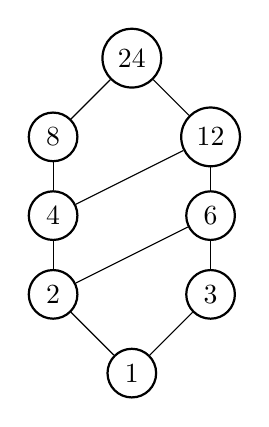
\begin{tikzpicture}
		\begin{scope}[every node/.style={circle,thick,draw}]
		    \node (1) at (0,0) {$1$};
		    \node (2) at (-1,1) {$2$};
		    \node (3) at (1,1) {$3$};
		    \node (4) at (-1,2) {$4$};
		    \node (6) at (1,2) {$6$};
		    \node (8) at (-1,3) {$8$};
		    \node (12) at (1,3) {$12$};
		    \node (24) at (0,4) {$24$};
		\end{scope}
		
		\begin{scope}[>={Stealth[black]},
		              every node/.style={fill=white,circle},
		              every edge/.style={draw=black}]
		    	\path (1) edge (2);
		    	\path (1) edge (3);
		    	\path (2) edge (4);
		    	\path (2) edge (6);
			\path (3) edge (6);
		    	\path (4) edge (8);
			\path (4) edge (12);
		    	\path (6) edge (12);
		    	\path (12) edge (24);
		    	\path (8) edge (24);
		\end{scope}
		\end{tikzpicture}
	\item The set of subsets of \{3,7\} with $\subseteq$ as a partial order.\\
		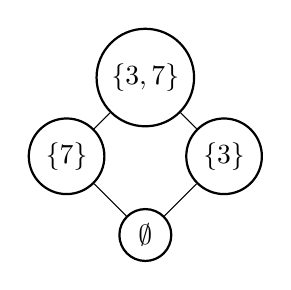
\begin{tikzpicture}
		\begin{scope}[every node/.style={circle,thick,draw}]
		    \node (empty) at (0,0) {$\emptyset$};
		    \node (7) at (-1,1) {$\{7\}$};
		    \node (3) at (1,1) {$\{3\}$};
		    \node (3-7) at (0,2) {$\{3,7\}$};
		\end{scope}
		
		\begin{scope}[>={Stealth[black]},
		              every node/.style={fill=white,circle},
		              every edge/.style={draw=black}]
		    	\path (empty) edge (3);
		    	\path (empty) edge (7);
		    	\path (3) edge (3-7);
		    	\path (7) edge (3-7);
		\end{scope}
		\end{tikzpicture}
	\end{enumerate}
\setcounter{enumi}{14}
\item Define the relations $<,\leq,\preceq$ on the plane $\R\times\R$ by\\
$(x,y)<(z,w)$ if $x^2+y^2<z^2+w^2$,\\
$(x,y)\leq(z,w)$ if $(x,y)<(z,w)$ or $(x,y)=(z,w)$,\\
$(x,y)\preceq(z,w)$ if $x^2+y^2\leq z^2+w^2$.
	\begin{enumerate}
	\item Which of these relations are partial orders? Explain.\\
	$\leq$ is a partial order. $<$ is not a partial order because it is not reflexive. $\preceq$ is not a partial order because 
	if $(x,y)=(0,1)$ and $(z,w)=(1,0)$ then $0^2+1^2=1^2+0^2$ so $x^2+y^2 = z^2+w^2$ so $(x,y)$ is related to $(z,w)$ and $(z,w)$ 	is related to $(x,y)$ but $(x,y)\not=(z,w)$ thus $\preceq$ is not antisymmetric.
	\setcounter{enumii}{2}
	\item Draw a sketch of $\{(x,y):(x,y)\leq (3,4)\}$.\\
		\begin{tikzpicture}
			\draw[dashed] (0,0) circle (2cm);
			\draw[thick,fill] (1,1.75) circle (0.15cm);
		\end{tikzpicture}
	\item Draw a sketch of $\{(x,y):(x,y)\preceq (3,4)\}$.\\
		\begin{tikzpicture}
			\draw[dashed] (0,0) circle (2cm);
			\draw[thick,fill] (1,1.75) circle (0.15cm);
		\end{tikzpicture}
	\end{enumerate}
\setcounter{enumi}{0}
\item Draw a Hasse diagram for $S=\{4,6,8,12\}$ with the partial order $\mid$.\\
	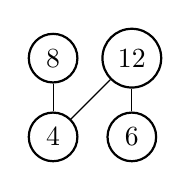
\begin{tikzpicture}
	\begin{scope}[every node/.style={circle,thick,draw}]
	    \node (4) at (0,0) {$4$};
	    \node (6) at (1,0) {$6$};
	    \node (8) at (0,1) {$8$};
	    \node (12) at (1,1) {$12$};
	\end{scope}
	
	\begin{scope}[>={Stealth[black]},
	              every node/.style={fill=white,circle},
	              every edge/.style={draw=black}]
	    	\path (4) edge (8);
		\path (4) edge (12);
	    	\path (6) edge (12);
	\end{scope}
	\end{tikzpicture}
\end{enumerate}

%SECTION 11.2
\section*{11.2}
\begin{enumerate}
\item Draw a Hasse diagram for the given order on $S\times T$, where $S=\{4,6,8,12\}$ with the partial order $\mid$, and $T=\{2,3,5\}$ with the partial order $\leq$. 
	\begin{enumerate}
	\item the product order\\
		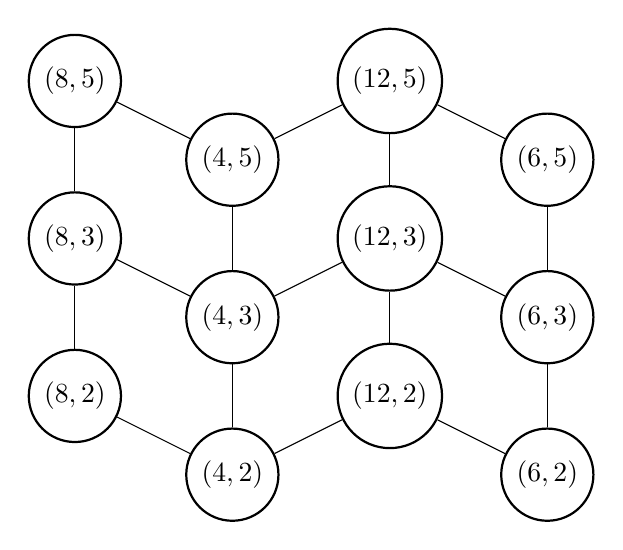
\begin{tikzpicture}
		\begin{scope}[every node/.style={circle,thick,draw}]
		    \node (4-2) at (0,0) {$(4,2)$};
		    \node (4-3) at (0,2) {$(4,3)$};
		    \node (4-5) at (0,4) {$(4,5)$};
		    \node (6-2) at (4,0) {$(6,2)$};
		    \node (6-3) at (4,2) {$(6,3)$};
		    \node (6-5) at (4,4) {$(6,5)$};
		    \node (8-2) at (-2,1) {$(8,2)$};
		    \node (8-3) at (-2,3) {$(8,3)$};
		    \node (8-5) at (-2,5) {$(8,5)$};
		    \node (12-2) at (2,1) {$(12,2)$};
		    \node (12-3) at (2,3) {$(12,3)$};
		    \node (12-5) at (2,5) {$(12,5)$};
		\end{scope}
		
		\begin{scope}[>={Stealth[black]},
		              every node/.style={fill=white,circle},
		              every edge/.style={draw=black}]
		    	\path (4-2) edge (4-3);
			\path (4-3) edge (4-5);
			\path (4-2) edge (8-2);
			\path (4-3) edge (8-3);
			\path (4-5) edge (8-5);
			\path (4-2) edge (12-2);
			\path (4-3) edge (12-3);
			\path (4-5) edge (12-5);
			\path (6-2) edge (6-3);
			\path (6-3) edge (6-5);
			\path (6-2) edge (12-2);
			\path (6-3) edge (12-3);
			\path (6-5) edge (12-5);
			\path (8-2) edge (8-3);
			\path (8-3) edge (8-5);
			\path (12-2) edge (12-3);
			\path (12-3) edge (12-5);
		\end{scope}
		\end{tikzpicture}
	\item the lexicographic order\\
		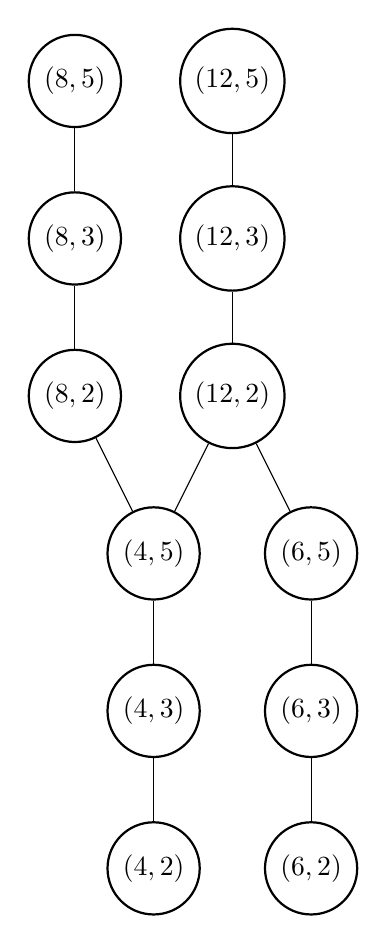
\begin{tikzpicture}
		\begin{scope}[every node/.style={circle,thick,draw}]
		    \node (4-2) at (0,0) {$(4,2)$};
		    \node (4-3) at (0,2) {$(4,3)$};
		    \node (4-5) at (0,4) {$(4,5)$};
		    \node (6-2) at (2,0) {$(6,2)$};
		    \node (6-3) at (2,2) {$(6,3)$};
		    \node (6-5) at (2,4) {$(6,5)$};
		    \node (8-2) at (-1,6) {$(8,2)$};
		    \node (8-3) at (-1,8) {$(8,3)$};
		    \node (8-5) at (-1,10) {$(8,5)$};
		    \node (12-2) at (1,6) {$(12,2)$};
		    \node (12-3) at (1,8) {$(12,3)$};
		    \node (12-5) at (1,10) {$(12,5)$};
		\end{scope}
		
		\begin{scope}[>={Stealth[black]},
		              every node/.style={fill=white,circle},
		              every edge/.style={draw=black}]
		    	\path (4-2) edge (4-3);
			\path (4-3) edge (4-5);
			\path (4-5) edge (8-2);
			\path (8-2) edge (8-3);
			\path (8-3) edge (8-5);
			\path (4-5) edge (12-2);
			\path (6-2) edge (6-3);
			\path (6-3) edge (6-5);
			\path (6-5) edge (12-2);
			\path (12-2) edge (12-3);
			\path (12-3) edge (12-5);
		\end{scope}
		\end{tikzpicture}
	\end{enumerate}
\end{enumerate}


\end{document}